\documentclass[a4paper]{IEEEtran}
 
\usepackage{amsmath}
\usepackage{graphicx}
\usepackage{caption}
\usepackage{subfigure}
\usepackage{epstopdf}
\usepackage[ansinew]{inputenc}
\usepackage{listings}
\usepackage{xcolor}
%\setlength{\oddsidemargin}{0cm}
%\setlength{\evensidemargin}{0cm}
%\setlength{\topmargin}{0cm}

\usepackage[]{algorithm2e}

\usepackage{a4wide}

\title{ Allen mouse brain circuit - visual debugging }
%\author{Till Schumann}
%\date{}

\begin{document}
   \maketitle
   
   \section{Description}
   A simulation of a full scale point neuron circuit of the mouse brain make great demands on the simulator, circuit generation and the used data formats.
   
Allen Institute for Brain Science provides a high-resolution map of neural connections in the mouse brain.
   It contains several injection experiments. The provided datasets of the experiments 
   contain a 3D volumetric data of the injection and a 3D volumetric data of its axonal projection labeled by viral
   tracers. Based on this data the long range connections for the point neuron circuit of the mouse brain are generated.   
   
   The full point neuron circuit contains $75e6$ neurons with around $1e4$ synapses per neuron.
   To make such a large scale simulation possible, we had to adapt the process from generating the point neuron circuit to extend the import functionality of NEST. Therefore we ported the circuit generation to a hybrid c++ application which can be executed on 2 racks of the IBM Blue Gene Q. It generates a big hdf5 file which contains all synapses information.
   To import the circuit into NEST, we implemented a module that allows to load the synapse information from the hdf5 file.
   
   To validate the generated circuit we would like to visualize the connections (source and target neurons) after the generation and the resulting spiking activity form the NEST simulation for a single experiment. 
   
   \section{Given data}
   \begin{itemize}
      \item x,y,z coordinates of neurons in hdf5 file
      \item synapses (source and target neuron ids) in hdf5 file
	  \item 3D volumetric injection and projection densities with $100\mu m$ voxel resolution in NRRD format
	  (http://help.brain-map.org/display/mouseconnectivity/API\#API-3DReferenceModels)
	  \item 3d volumetric number of neurons per voxel with with $100\mu m$ resolution (C style, int values)
   \end{itemize}
   
   \section{Work-flow}
   For debugging the circuit is generated for a single experiment. Thus there are only connections
   from neurons inside the injection area to neurons inside the projection area. In a first step the injection area , the projection area ,all source and target neurons should be visualized in a 3D raster. In a second step this circuit is simulated with NEST with a high stimulus to all neurons inside the injection area. The activity should be visualized in a 3D raster, still showing the injection and projection area. If there is only spiking activity in this region the circuit generation and the import module work fine.
   
   \begin{figure}[ht!]
   	\begin{center}
        \subfigure[Injection sites - showing all available experiments]{%
            \label{fig:allInjections}
            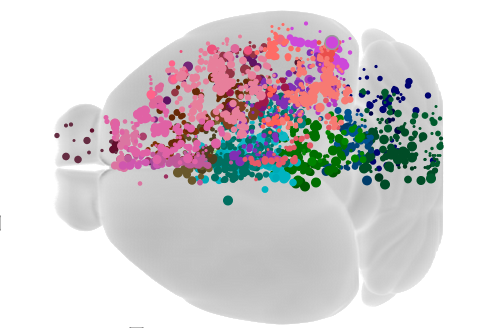
\includegraphics[width=0.4\textwidth]{../connectionBrowser_allinjections.png}
        }
        \hspace{1cm}
        \subfigure[Projection of one experiment]{%
            \label{fig:oneProjection}
            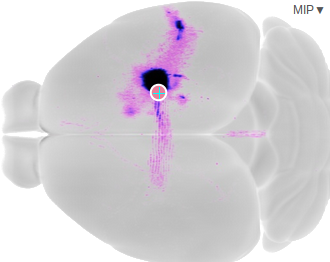
\includegraphics[width=0.32\textwidth]{../connectionBrowser_oneinjections.png}
       }
    	   \end{center}
    	\caption{%
        The pictures are inverted and copied from the Allen Brain Atlas.
     }%
   \label{fig:atlas}
   \end{figure}
   
   \begin{figure}[ht!]
   	\begin{center}
        \subfigure[Number of excitatory neurons per voxel]{%
            \label{fig:allInjections}
            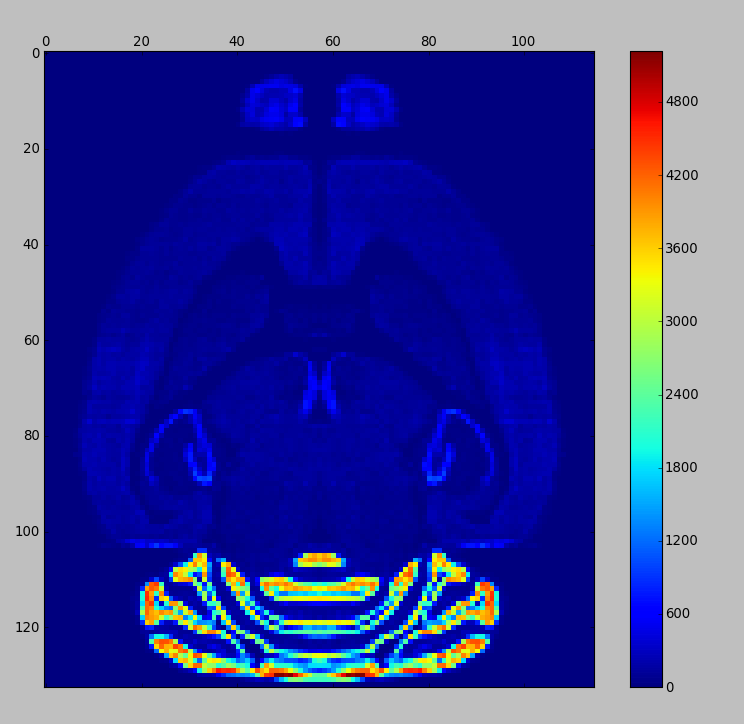
\includegraphics[width=0.4\textwidth]{../exNeurons_numPerVoxel.png}
        }
        \hspace{1cm}
        \subfigure[Illustration of neurons inside an injection and projection area]{%
            \label{fig:oneProjection}
            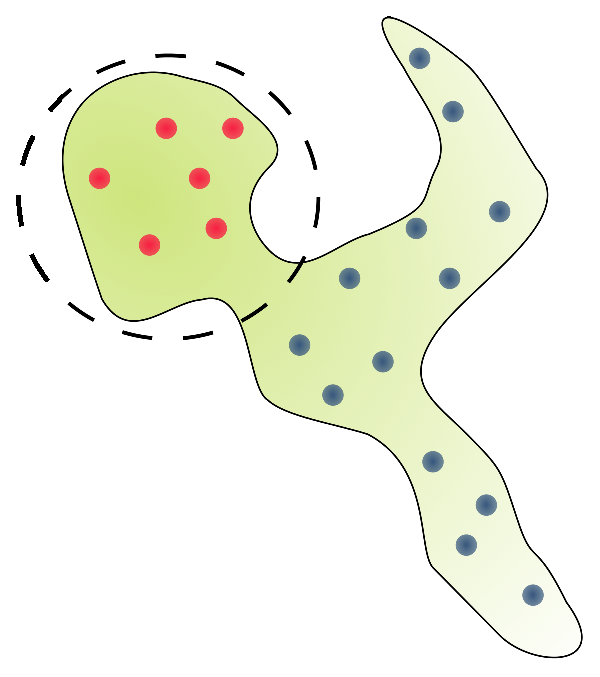
\includegraphics[width=0.35\textwidth]{drawing.eps}
       }
    	   \end{center}
    	\caption{%
        The plots (x vertical and z horizontal axis) show a slice (along the y axis) of the 3D datasets. 
     }%
   \label{fig:atlas}
   \end{figure}
   \newpage
	
	
	

\end{document}
